\documentclass{template}
\usepackage{graphicx,parskip,float}
\usepackage[ruled] {algorithm2e}
\usepackage{url,amsmath,amssymb,fancybox,listings,pdfpages,caption,multicol,datetime,rotating, booktabs}

%\usepackage[usenames,dvipsnames]{color}
\usepackage[pagebackref=false,pdffitwindow=true]{hyperref}
\usepackage{apacite}
%NOTE: The hyperref usepackage should be the last \usepackage!!
%NOTE: When pagebackref=true an error will appear at the end of compiling. press `q' to ignore
%NOTE: Referencing Algorithms does not work if this usepackage is before the hyperref include.!!
%NOTE: This is a comment, ignored when the document is compiled
%NOTE: The following document configuration settings generally do not need to be modified
%NOTE: More packages may need to be added to provide additional functionality



\hypersetup{
    pdftitle    = {Report Title},
    pdfauthor   = {Author Name},
    pdfsubject  = {Subject Area},
    pdfkeywords = {Comma separated list of keywords},
    colorlinks  = true, anchorcolor = blue, filecolor = blue, urlcolor = blue,
    linkcolor   = blue,    %NOTE: change (blue) to (colIdentifier) to have links within the document in Black
    citecolor   = blue,    %NOTE: change (blue) to (colIdentifier) to have citation links within the document in Black
}

\definecolor{colBackGrnd}{rgb}{1,1,0.8}
\definecolor{colKeys}{rgb}{0,0,1}
\definecolor{colIdentifier}{rgb}{0,0,0}
\definecolor{colComments}{rgb}{0,.5,0}
\definecolor{colString}{rgb}{0,0,1}
\definecolor{colWhite}{rgb}{1,1,1}

\newcommand{\MyHookSign}{\hbox{\ensuremath\hookleftarrow}}

\newtheorem{Theorem}{Theorem}
\newtheorem{Proposition}[Theorem]{Proposition}
\newtheorem{Lemma}[Theorem]{Lemma}
\newtheorem{Proof}[Theorem]{Proof}
\newtheorem{Remark}[Theorem]{Remark}
\newtheorem{Claim}[Theorem]{Claim}
\newtheorem{Example}[Theorem]{Example}
\newtheorem{Definition}[Theorem]{Definition}

%NOTE: Setup for including program listings
\lstset{%
    float=H,
    basicstyle=\ttfamily\footnotesize,
    identifierstyle=\color{colIdentifier},
    keywordstyle=\color{colIdentifier}, %
    stringstyle=\color{colIdentifier},
    commentstyle=\color{colIdentifier}, %
    columns=flexible,
    tabsize=2,
    frame=single,
    extendedchars=true, %
    showspaces=false,
    showstringspaces=false,
    numbers=left, %
    numberstyle=\footnotesize,
    breaklines=true,
    prebreak={\space\MyHookSign},
    language=Java,
    backgroundcolor=\color{colBackGrnd},
    breakautoindent=true, %
    captionpos=b%
} %\hypersetup{colorlinks=true, citecolor=\color{colIdentifier}}

\sloppy %NOTE: To ensure the Right Hand Margin is used (Especially for long URLS)
%NOTE: END of the document configuration settings

\begin{document}

\DeclareGraphicsExtensions{.jpg,.png,.gif,.pdf}
%NOTE: When inserting Figures if the extension of the graphic file is not provided LaTeX will automatically search
% for the extensions declared above, in the order declared.

\title{\huge{Using Deep Learning to Analyse X-Rays}}
\author{Jehanzeb Mobarik}
\degreetitle{BSc in Computer Science} % Replace with appropriate degree
\rpttype{BSc}    % Replace MSc with BSc for Honours Degree Year projects.
\principaladviser{Dr. Eyad Elyan}

\include{intro/abstract}


%NOTE: Include the relative reference for each chapter to be included
% dividing the thesis file structure into a number of directories aids development
% format: directoryName/filename (the .tex extension is not required for the filename)




\chapter{Literature Review}
This chapter is a review of the relevant literature around deep learning and how this type of machine learning has advanced in the past years . In particular, the report will discuss how deep learning can be used in the diagnosis of pathologies in chest X-rays. As well as this we will review successful projects from the past that are closely linked to this thesis.

\section{Overview}

Radiology is a branch of medicine which uses medical imaging technology to generate images so that radiologists can view structures within the human body. The types of images range from X-rays, CT scan(computed tomography scan) and ultrasounds. \cite{bradley2008history}. For the past few years, radiology in the UK  has seen disruption in the National Health Service. A reoccurring issue amongst radiology departments is lack of staff to interpret scans. According to the Royal College of Radiologists, the NHS does not have enough radiologists to meet diagnostic imaging demands leaving patients at risk. \cite{rimmer2017radiologist}. 
\space
\subsection{Faster Diagnosis}
One area which can augment the diagnosis of medical scans is image classification. This process of image classification involves teaching a model to learn features from images and then test on unseen images to compute accuracy. In recent times, image classification through deep learning methods has produced  superhuman performance on several image-based classification tasks\cite{krizhevsky2012imagenet}.
\section{Traditional Methods of Machine Learning}
Before the advancements in deep learning, less sophisticated methods of image classification were employed. This method of machine learning required the crucial step of feature extraction before inputting data into a classifier. In order to visualise the process that needs to take place when using traditional methods of machine learning please refer to figure~\ref{fig:FeatureExtraction}.


	

\begin{figure}[H]
	\centering
	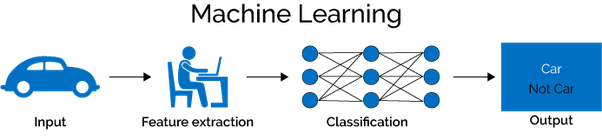
\includegraphics[scale=0.5]{MachineLearningvsDeepLearning.png}
	\caption{Figure showing the process of traditional image classification using feature extraction(Image taken from TowardsDataScience)}
	\label{fig:FeatureExtraction}
\end{figure}


 Computers see images as pixel values, and each image can be viewed as a 2D matrix of pixel values. When building a machine learning pipeline to classify an image, we need to be able to tell what is unique about each image so that the classifier shown in figure~\ref{fig:FeatureExtraction} can correctly classify. This uniqueness in an image can also be viewed as the features. Classification can then be thought of as detection of features in an image, and if features associated with a class are present in the input, we can predict if the input image is of a specific class \cite{MIT.2019}


 In order to build a classification pipeline, the model needs to know what features it is looking for in an input image. These features it is looking for are a predefined set of features. In order to apply this rule, we can leverage human knowledge about a picture in a given domain and extract the most important features. We can then detect those manual features and use that detection to make a classification prediction \cite{popescu2014feature}

 However, images can have lots of variation. If we want to build a robust pipeline, our model needs to be invariant to image variation, while still being sensitive to the differences in individual classifications. Manual features defined by humans can be used, but where this manual detection breaks down is in the detection task itself, and this is merely based on the fact that one class can have incredible amount of variation. This can be illustrated with the ~\ref{fig:FeatureExtractionIssue} provided by \cite{szegedy2015going}
 
 \begin{figure}[H]
 	\centering
 	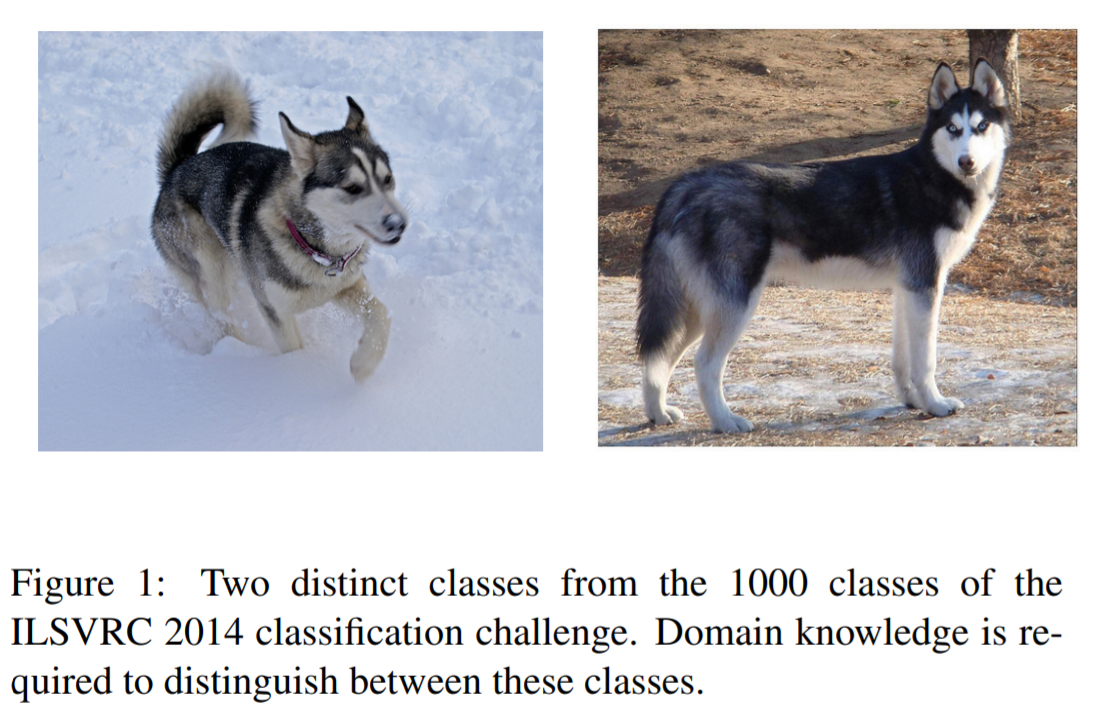
\includegraphics[scale=0.5]{DomainKnowledgeIssueGoogleNet.png}
 	\caption{Two distinct class from 1000 classes of the ImageNet database. Domain knowledge is required to distinguish between separate classes}
 	\label{fig:FeatureExtractionIssue}
 \end{figure}
 

 So, how can we do better? We want a way to both extract features and detect their presence in an image automatically. This is where deep learning can be harnessed to extract features, no matter how the image is presented, automatically.
\section{State-of-the-Art}

Convolutional Neural Networks are a special kind of Multi-layered Perceptron(MLP). Like almost every other neural network they are trained with a version of back-propagation algorithm. Where they differ is in the architecture. This contrast can be viewed in figure~\ref{fig:MLP} and figure~\ref{fig:CNN}. CNN's are designed to recognise visual patterns directly from pixel values with minimal preprocessing. They can recognise patterns with extreme variability(such as handwritten characters) and with robustness to distortions and simple geometric transformations. \cite{lecun1989backpropagation}
CNN's differ from MLP's in that they take advantage of spatial information of an image by convolving a patch of the input image with a filter weight of the same dimension. This results in a 2D matrix called a feature map. These filter weights are applied over the whole image and are iteratively refined in the training process , so that the correct features can be extracted. Different weight filter can be used to extract different features. This is achieved by passing the input across multiple convolution layers. In order to visualise this please refer to figure ~\ref{fig:CNN}. From the diagrams it can be appreciated that MLP's lose all spatial information about an image by flattening every pixel and connecting these pixel values to a neuron in the hidden layer. As well as this we can see that MLP's have many more parameters in the network compared to CNN which can lead to over-fitting especially if the number of training samples is limited. \cite{szegedy2015going}
Starting with LeNet-5 , CNNS's have typically had a standard stacked structured of convolutional layers, followed by ReLU operation, max-pooling and then a fully connected layer. There are variants of this basic design in different image classification tasks and they have all yielded respective results on classification tasks such as MNIST and CIFAR. Although, the most notable includes the ImageNet classification challenge where 1.2 million images were classified into 1000 different classes. In the past years CNN architectures have dominated this challenge and the first publication using CNN architecture was produced by Alex Krizhevsky and Geoffery Hinton in 2012\cite{krizhevsky2012imagenet}. The architecture was given the name Alex-Net and achieved a top-5 error rate of 15.3\% outperforming the previous state-of-the-art, SIFT \cite{lowe2004distinctive} which achieved a 26.2\% error rate using traditional methods. Since then, new CNN architectures have been published with improved results and this can be seen in the table below. 

\begin{figure}[H]
	\centering
	\includegraphics[scale=0.5]{MLP.png}
	\caption{Architecture for MLP. Shows how all pixels value in image are flattened losing all spatial infromation(\url{https://alexlenail.me/NN-SVG/index.html})}
	\label{fig:MLP}
\end{figure}


\begin{figure}[H]
	\centering
	\includegraphics[scale=0.5]{CNN.png}
	\caption{Architecture for Le-Clun CNN. Shows how spatial information is preserved as well different operations applied (\url{https://alexlenail.me/NN-SVG/LeNet.html})}
	\label{fig:CNN}
\end{figure}

\begin{table}[H]
	\centering
	\small
	\begin{tabular}{llll}
		\toprule 	Model & Top-5 error rate &Number of Layers\\
		\midrule
		AlexNet(2012)  & 15.3\%	&  8 layers\\
		VGG16(2014)&7.3\%  & 19 layers\\
		GoogleNet(2014)&6.7\% & 50 layers\\
		InceptionV3(2015)&3.58\%& 50 layers\\
		ResNet(2015)    &3.57\% &152 layers\\
		\bottomrule
	\end{tabular}


	\caption{Results of different models with Human error rate at 5.1\%}\label{tab:Results}
\end{table}




From the table we can see that for large datasets such as ImageNet, there is seems to be a trend developing. That is that the number of layers as well as layer size is increasing. A bigger size means that the model holds more parameters and can make it more prone to over-fitting. To address this problem, a technique developed by Goolge called ``dropout" was developed \cite{hinton2012improving}

\section{Related Work}

Many papers have been published in the domain of using deep learning for medical image analysis. This has been spurred in part due to large carefully curated labelled datasets which have led to papers showing expert-level performance on many medical image classification tasks \cite{irvin2019chexpert}. In this section we will review work related to the thesis title. 


\setcounter{secnumdepth}{4}

\subsection{CheXNet}
In this project, led by Stanford ML Group, an algorithm was developed to interpret chest X-ray images and detect if Pneumonia is present while showing a heat map of the area in the image that had the highest activations \cite{rajpurkar2017chexnet}. Example output can be see in figure~\ref{fig:CheXNetExample}


\begin{figure}[H]
	\centering
	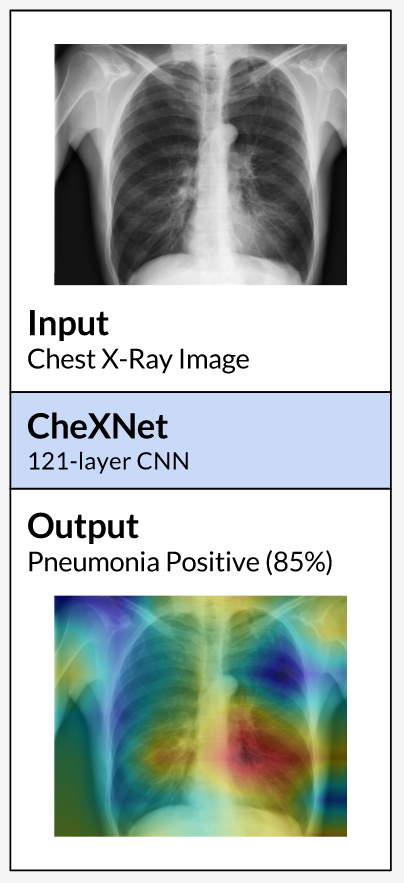
\includegraphics[scale=0.5]{HeatMap.png}
	\caption{Example of CheXNet output of class label along with probability from softmax layer and heat-map}
	\label{fig:CheXNetExample}
\end{figure}

Results showed that the algorithm can detect the pathology at a level exceeding radiologists. The algorithm used a 121-layer CNN which was trained on ChestX-ray14 \cite{wang2017chestx} which is currently the largest publicly available chest X-ray dataset, containing over 100,000 frontal view images and 14 different pathologies. The CNN used is based on the DenseNet architecture \cite{huang2017densely} but modifications were made for single output in the fully connected layer by applying a non-linearity sigmoid function, so that only Pneumonia would have a probability. Pre-trained weights were initialised from a model trained on ImageNet \cite{deng2009imagenet} to speed up the process of training. 
\subsubsection{Results}
Precautions were put in place to make sure that patient images between training and testing sets never overlap. In order to test the accuracy of the model, 420 chest X-rays were collected and 4 practising radiologists annotated where they think the Pneumonia is present. Through the CheXNet tests it showed the algorithm exceeds average radiologist performance on the \textbf{F1 metric}. The model was comparative with expert radiologists on metrics such as \textbf{accuracy}, \textbf{sensitivity} and \textbf{specificity}. The biggest difference was in terms of speed as radiologists took around 4 hours on average to interpret the images whereas CheXNet algorithm took less than 2 minutes \cite{rajpurkar2017chexnet}. Results from figure~\ref{fig:F1Score} present the F1 score for algorithm and average of the 4 clinicians. 

\begin{figure}[H]
	\centering
	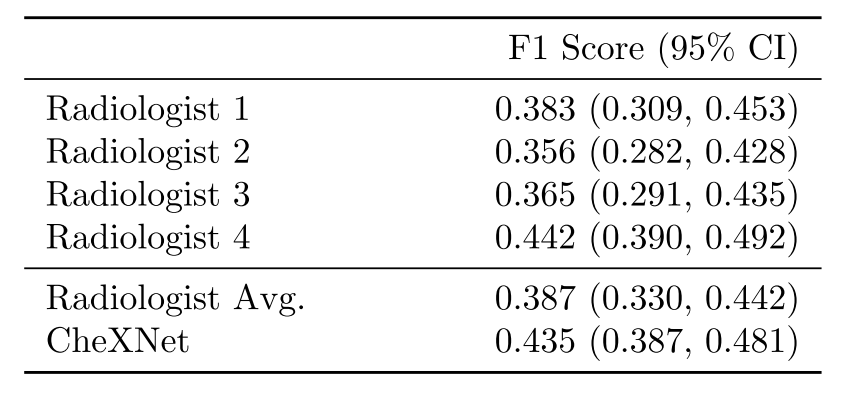
\includegraphics[scale=0.5]{F1Score.png}
	\caption{F1 Score for CheXNet and average F1 score for 4 radiologists}
	\label{fig:F1Score}
\end{figure}
\setcounter{secnumdepth}{4}
\subsection{Multi-task Learning for Chest X-ray Abnormality}
In this paper, researchers built a model trained on 297,541 chest X-rays. The system is based on a novel multi-task deep learning architecture that in addition to classifying and showing a heat-map of the abnormalities also supports the segmentation of the lungs and heart \cite{guendel2019multi}. The research demonstrated that by training the model concurrently on these tasks, one can increase the classification performance. This research produced state of the art performance of 0.883 AUC on average across 12 different abnormalities. ChestX-Ray 14 \cite{wang2017chestx} and PLCO datasets were combined to increase the amount of variability of images and this also showed increase in performance. 

As mentioned before techniques were applied to increase accuracy. One of the methods employed was to normalise the images. A challenge in processing chest radiographs is that there can be large variabilities in the appearance of the image and this is due to the acquisition source, radiation dose \cite{guendel2019multi}. The paper proposes to dynamically window each image by adjusting the brightness and contrast via a linear transformation of the image intensities. Example of output is shown in figure~\ref{fig:Normalisation} 


\begin{figure}[H]
	\centering
	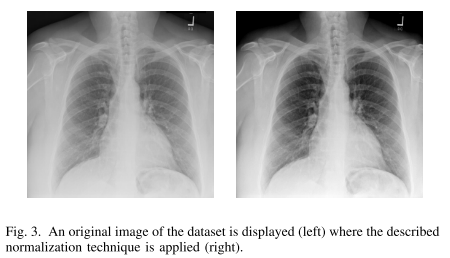
\includegraphics[scale=0.7]{NormalisationTechnique.png}
	\caption{We can see that certain parts of the X-ray become more visible hence making abnormalities more clear for the model}
	\label{fig:Normalisation}
\end{figure}

In addition , the paper also harnesses spatial knowledge related to individual pathologies as well as underlying structure i.e the heart and lungs which can be exploited to increase classification performance. The paper proposes that once can focus the learning task to the heart and lung region as information outside of these regions may be regarded as irrelevant for the diagnosis of heart/lung abnormalities. 

In order to achieve this segmentation, a DenseNet model shown in figure~\ref{fig:DenseNet} \cite{huang2017densely} has been used and figure~\ref{fig:Segmentation}  presents the architecture as well as an example showing the segmentation technique. Another technique that was used to take advantage of spatial information was the use of several approximate spatial labels provided in the PLCO dataset. For five abnormalities(Nodule,Mass,Infiltrate,Atelectasis,Hilar Abnormality) there are rough location information available  to help the model locate where the abnormality is usually located.



\begin{figure}[H]
	\centering
	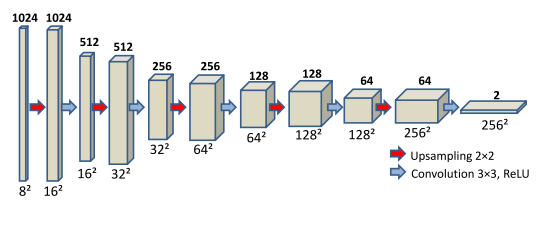
\includegraphics[scale=0.7]{DenseNet_Architecture.png}
	\caption{Architecture for DenseNet}
	\label{fig:DenseNet}
\end{figure}

\begin{figure}[H]
	\centering
	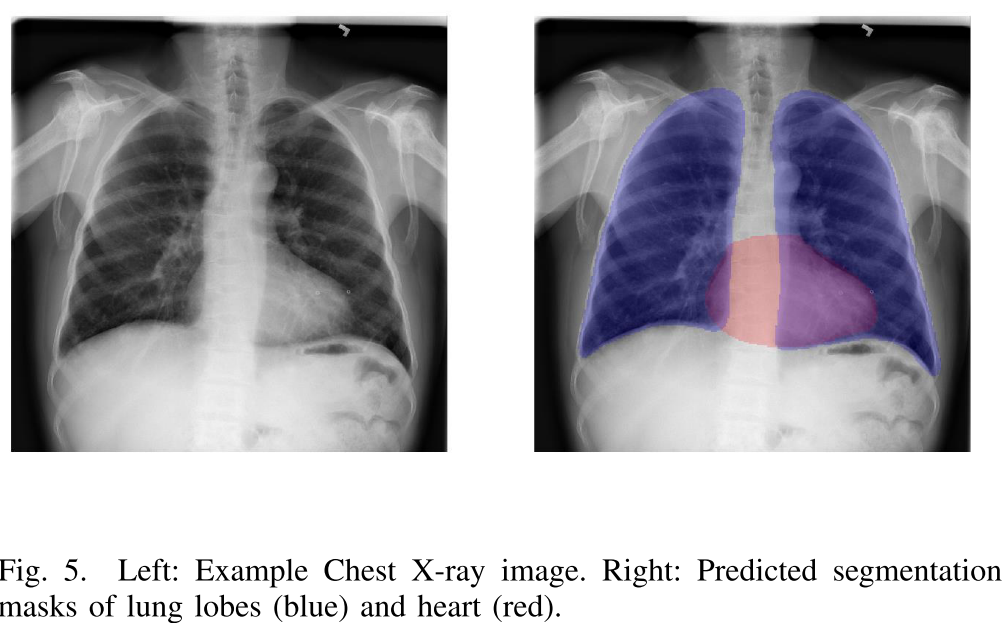
\includegraphics[scale=0.4]{Segmentation.png}
	\caption{Distinct segmentation of lungs and heart}
	\label{fig:Segmentation}
\end{figure}



\subsubsection{Results}


For this paper, different experiments were undertaken to show the performance of the model. As a baseline, performance was measured by only training the classification part on the PLCO dataset. The test was evaluated with an average \textbf{AUC} score across 12 abnormalities of \textbf{0.859}. \par
Results also showed improved classification scores when the network was additionally trained to generate lung and heart segmentation masks (as shown in  figure~\ref{fig:AUC}). Performance increased to 0.866 on average across the abnormalities. \par
As mentioned another technique was to use spatial knowledge and the impact of this showed an average improvement of 0.011\par
This paper also used 2 datasets and by combining both, the average AUC score reaches 0.870. This increase in score is due to more variability in the learning process. As well as this the normalisation technique previously shown in figure~\ref{fig:Normalisation} was applied when training the model and this had a 2 fold benefit. The first was that the training process was reduced on average 2-3 times. The researchers hypothesised that this is due to the images being more aligned in terms of brightness and contrast. Another reason was due to the generalisation of the model parameters and this lead to a performance gain of 0.876. \par
Finally, the researchers upscaled the input image size to 512 in each dimension and adjusted the DenseNet layer to take in 16x16 patch size at each layer. This final network architecture change also added all of the previous techniques mentioned before. The following image shows the results obtained across all techniques and finally the result of combining all the techniques which produces a state-of-the-art performance of \textbf{0.883}



\begin{figure}[H]
	\centering
	\includegraphics[scale=0.4]{AUC_Scores.png}
	\caption{Results showing increasing mean AUC score}
	\label{fig:AUC}
\end{figure}
\setcounter{secnumdepth}{4}
\subsection{Abnormality Detection and Localization in Chest X-Rays using Deep Convolutional Neural Networks}

For this paper, researchers conducted experiments on three datasets. From the datasets, researchers explored the performance of various deep CNN's for detection of heart disease from chest X-rays. Researchers used binary classification on diseases such as Cardiomegaly against normal images \cite{islam2017abnormality}. The paper explores several CNN models such as AlexNet, VGG-Net and ResNet. These models have different layers and typically achieve higher accuracy as layers increase as noted in State-of-the-Art section.

Another part of the research, similar to previous papers reviewed was to produce a heat-map showing which areas of the X-ray the model has the highest activation on. This paper used the sensitivity of softmax scores of occlusion on a certain region in the chest X-ray to find which region in the image is responsible for the classification decision.  
\subsubsection {Results}

The first experiment used single model CNN's on the Indiana dataset, and from the tests, it was shown that deeper models like VGG-19, ResNet improve the accuracy significantly. It was found that Cardiomegaly detection improves 6\% compared to using shallower models like AlexNet. Although results showed high specificity for ResNet-101 and high sensitivity for VGG-16, the VGG-19 gave the highest AUC score of 0.94. This at least 1\% higher AUC for other models. 
As well as this, dropout was used, which increased performance on the shallower networks but degraded deeper ones. For all experiments, it was noted that extracting features from earlier layers lead to improved accuracy of 2-4\%. It was concluded that shallower networks were better for detecting smaller objects, and as an example, it was found that shallower layers from ResNet-15 trained on Cardiomegaly had better performance than later layers across different metrics. figure~\ref{fig:Shallow} shows a more in depth picture of findings. 

\begin{figure}[H]
	\centering
	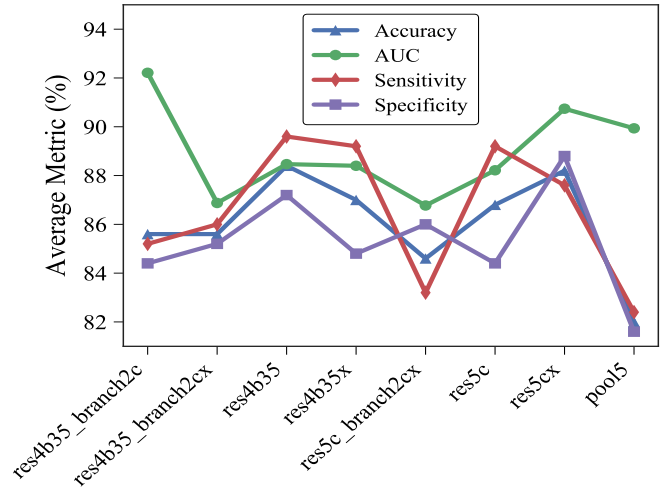
\includegraphics[scale=0.7]{ShallowerLayers.png}
	\caption{Researchers showed that shallower layers in models had a higher accuracy on Cardiomegaly detection compared to deep layers}
	\label{fig:Shallow}
\end{figure}

Another fascinating result was on the localisation of Cardiomegaly shown in the image below. It can be observed that from the figure~\ref{fig:Cardiomegaly}, the model has higher activations from the heart region, which is expected as Cardiomegaly concerns abnormal enlargement of the heart. What was revealing was that other than an enlarged heart for a patient with Cardiomegaly, there is not much difference in features between a normal image and an image classified as Cardiomegaly. But the model can still differentiate between a normal heart which is enlarged due to age or physical attributes of the patient. 
\begin{figure}[H]
	\centering
		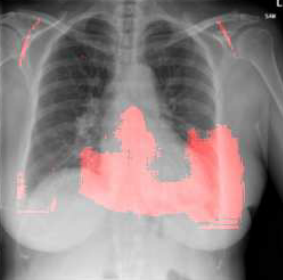
\includegraphics[scale=0.7]{CardiomegalyMap.png}
	\caption{Occlusion sensitivity used to create heap map of region where it thinks Cardiomegaly exists }
	\label{fig:HeatMap}
\end{figure}

\begin{figure}[H]
	\centering
	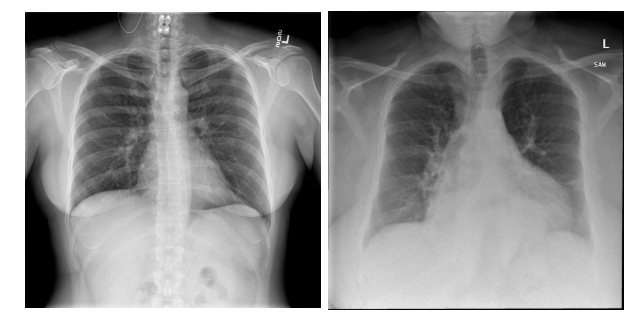
\includegraphics[scale=0.7]{NormalVsCardiomegaly.png}
	\caption{Example of normal heart on the left and Cardiomegaly diagnosed heart on the right }
	\label{fig:Cardiomegaly}
\end{figure}



Finally, another point raised in the paper was the model used for localisation of cardiomegaly were counter-intuitive to traditional methods of cardiomegaly diagnosis, which consider the relative size of heart and lung. But, most of the signals contributing to the softmax score come from the heart alone indicating features in the shape of the heart and its surrounding region alone help in detection of the pathology and perhaps the lung and relative size to the heart are less critical in the diagnosis for the model. 
 

 
 









\include{ActualThesis/ReviewOfRelatedWork}
\section{Medical Images}

As mentioned in the Overview section, radiology departments in the UK have struggled to meet imaging diagnostic demands. The survey published by the Royal College of Radiology reported 97\% of radiology departments were unable to do so within their working hours. As mentioned in the paper, ``It points to an insufficient number of radiologists to meet the increasing demand for imaging and diagnostic services". According to the report it cited that radiology has the second lowest proportion of trainees to consultants: 26 trainees to every 74 consultants. This is compared to an average in all specialities of 40 trainees for every 60 consultants. The report also cites that there was a particular workforce shortage prominent in Scotland, where the consultant workforce grew by 7\% from 2010 to 2016 but demand for CT,MRI scans increased by 10\%. 
One of the profound impacts of such shortage is the risk to patient care as well as economical effects. The NHS paid nearly £88m in 2016 for backlogs of radiology examinations to cover backlogs of radiology examinations to be reported. To cover these backlogs 92\% of radiology departments paid staff overtime, 78\% outsourced to private companies and 52\% employed ad hoc locums. This amount could have paid for at least 1028 full time radiology consultants.\cite{rimmer2017radiologist}

Given this what has been done to augment the analysis of medical images in the NHS and reduce extreme workload and large expenses ? One particular software which has bee used in the clinical setting is Computer Aided Diagnosis(CAD). CAD is technology which is designed to decrease observational oversights and false negative rates for physicians interpreting medical images such as mammographies \cite{castellino2005computer}. According Dr. Paul Chang, the reason this type of software did not receive as much attention, compared to the possibility of using deep learning, was that it used traditional methods of machine learning. \cite{youtube}

\subsection{Challenges}

There many challenges associated when applying new technologies in a clinical setting. Medical images are very large and complicated and for most of the image classification tasks in the ImageNet example , distinct features or pixels can be learned by a model. Dr. Matthew Lungren , radiologist at Stanford Medical Center, mentioned how most of the pixels in a chest X-Ray from a healthy person who happens to have lunge cancer , will tell you that the image is of a healthy person. But there is only a small proportion of the image which indicates the finding of lung cancer fo the classifier. Dr Lungren also noticed how medical images may have, what is known as artefacts or tokens in the image. Doctors are able to deal with context when looking at an image , but such artefacts or tokens may lead to a model making a decision with higher degree of confidence but in actual fact the classification is incorrect \cite{DrLungren.2018}


\section{Summary of Review}

From the review, it is quite evident that with the ever-growing concern in the NHS of a shortage of radiologists \cite{rimmer2017radiologist}, solutions need to be found in order to solve the issue of increased backlogs. Image classification, as mentioned, can provide augmentation of diagnosis of X-rays. Great leaps and bounds have been made in the field of deep learning and particularly well know CNN architectures show performance exceeding that of human intelligence in the case of ImageNet challenge \cite{krizhevsky2012imagenet}s. As well as this more sophisticated example of applying deep CNN's to medical images has shown outstanding results on pathologies such as Pneumonia and Cardiomegaly \cite{rajpurkar2017chexnet}. This problem of diagnosing X-rays also comes with its challenges which have been outlined in the challenges section. Other hurdles must be kept in mind for implementation purposes, and these include making sure that pixel values are not lost. Given the nature of X-rays, pixel loss can lead to pathologies being removed from an image such as lung nodules and according to the Royal  College of Radiologists certain rules needs to be adhered to so that images do not lose quality when it comes to diagnosing them. Lastly, when training a model on medical images, the dataset chosen needs to be balanced in class labels. As well as this one of the big obstacles is lack of datasets of reliable labelling of datasets as noise in class labels can lead to reduced performance. 


\section{Conclusion}

In this section, we will conclude how the rest of this thesis will be implemented and how the proposed problem in the introduction will be approached. From the findings above the aim is to apply one of the well known CNN architectures to build an accurate image classification pipeline on predicting the presence of Pneumonia in chest X-rays. In order to train the model, a carefully curated dataset must be chosen.  The dataset that will be used in this thesis comes from a public dataset carefully curated by Stanford ML Group called CheXPert. This dataset was created to solve three problems which include enough instances, strong reference standards and provide human performance metrics for comparison. It consists of 224,316 chest X-rays, and one of the main obstacles in the development of these datasets is the lack of strong radiologist-annotated ground truth.
The objectives is to build an accurate model which can predict and localise the Pneumonia with techniques such as occlusion. Another objective would be to build an interface which allows the entry of a chest X-ray and a predicted class label will be given back as well as a heat-map indicating which parts of the image had the highest activation. 
Lastly, if results from the initial pipeline show high accuracy, specificity, sensitivity and AUC, then the model could be extended to classify more than one pathology contained in the dataset.




\footnotesize  %NOTE: reduced the size of the text for the bibliography
%NOTE: set the style for the bibliography and display the references used within the document
\bibliographystyle{apacite}
\bibliography{ActualThesis/References}
\normalsize

\end{document} %NOTE: END of document, nothing after this point
